\documentclass{beamer}
%\documentclass[handout]{beamer}

%\usepackage{beamerjcf}
\usepackage[latin1]{inputenc}

\definecolor{kwblue}{rgb}{0.67,0.12,0.92}
\definecolor{ceruleanblue}{rgb}{0, 0.48, 0.65}
\definecolor{lightpink}{rgb}{1., 0.71, 0.75}
\definecolor{lightblue}{rgb}{0.8,0.8,1}
\definecolor{lightred}{rgb}{1,0.8,0.8}

\let\emph\alert

\begin{document}

\title{Map/Reduce for the common man}
\author[Jean-Christophe]{Jean-Christophe Filli\^atre \& Kalyan Krishnamani}
\institute{
}
\date{ProVal, February 19, 2010}

\begin{frame}
  \titlepage
  \pgfimage[height=8mm]{cnrs-logo2}\hfill
  \pgfimage[height=6mm]{saclay}\hfill
  \pgfimage[height=10mm]{lrilogo}\hfill
  \pgfimage[height=8mm]{upsudlogo}
\end{frame}

\begin{frame}\frametitle{Overview}
  \begin{enumerate}
  \item Google's Map/Reduce
  \item Ocaml's Map/Reduce
  \item Implementation details
  \end{enumerate}
\end{frame}

\begin{frame}\frametitle{Google's Map/Reduce}
  \begin{itemize}
  \item 
    what it is
    \begin{itemize}
    \item a paradigm for distributed computing at Google
    \end{itemize}

    \bigskip
  \item 
    what it offers
    \begin{itemize}
    \item abstraction to hide parallelization and distribution from
      user level code
    \end{itemize}

    \bigskip
  \item 
    application domains
    \begin{itemize}
    \item large scale data processing
    \end{itemize}
  \end{itemize}

  \vfill
  [MapReduce: Simplified Data Processing on Large Clusters. \par
  J. Dean and S. Ghemawat. OSDI 2004]
\end{frame}

\begin{frame}\frametitle{Main Idea}
  the user provides two functions
  \begin{itemize}
  \item \emph{map}: takes a key/value pair and returns a list of key/value
    pairs
    \begin{ocaml}
    map : k1 * v1 -> (k2 * v2) list
    \end{ocaml}



  \item \emph{reduce}: takes a list of values for one key and returns
    another list for that key
    \begin{ocaml}
    reduce : k2 * v2 list -> v2 list
    \end{ocaml}
  \end{itemize}



  and the library takes care of the rest
\end{frame}

\begin{frame}\frametitle{}
  \begin{center}
    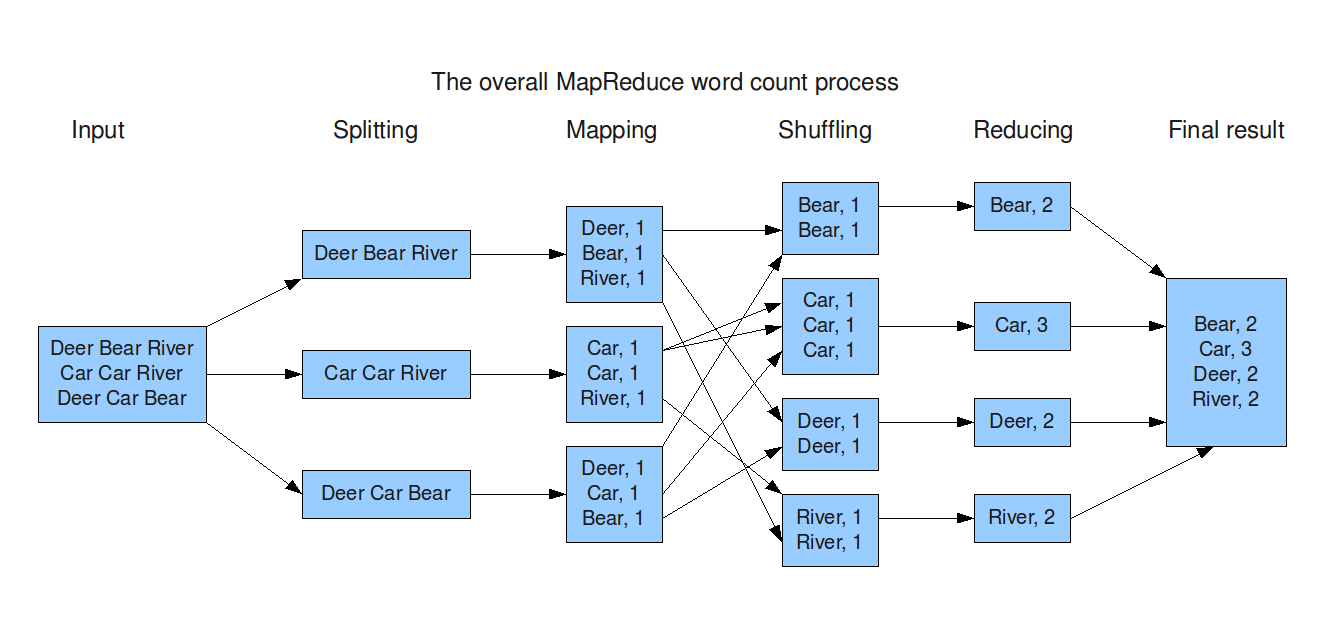
\includegraphics[width=\textwidth]{mrwordcount}
  \end{center}
\end{frame}

\begin{frame}\frametitle{}
  \begin{center}
    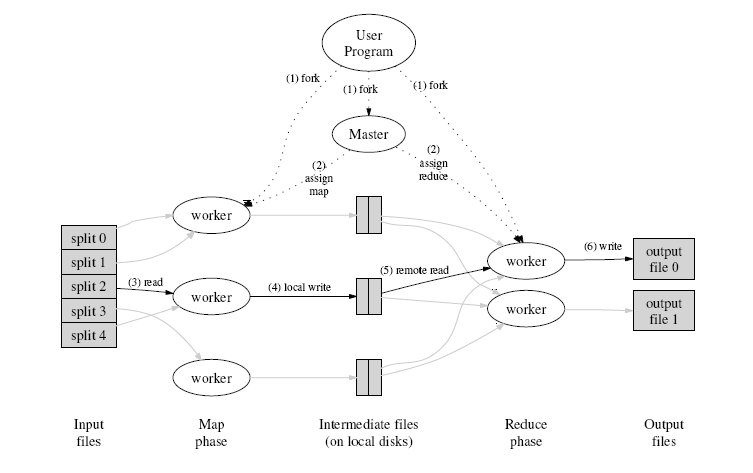
\includegraphics[width=\textwidth]{mrfigure}
  \end{center}
\end{frame}

\begin{frame}\frametitle{}
  \begin{center}
    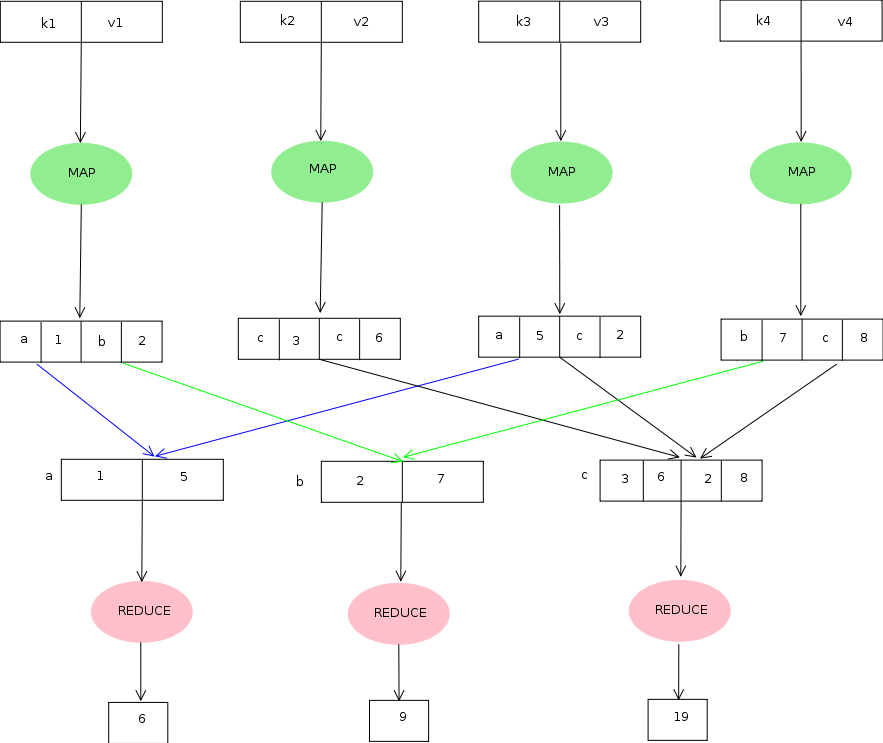
\includegraphics[width=\textwidth]{mr-new}
  \end{center}
\end{frame}

\begin{frame}
  \begin{center}
    \hrulefill\\
    \emph{Ocaml's Map/Reduce}
  \end{center}
\end{frame}

\begin{frame}\frametitle{Ocaml's Map/Reduce}
  \begin{itemize}
  \item 
    what it is
    \begin{itemize}
    \item a distributed computing library for Ocaml users
    \end{itemize}

    \bigskip
  \item 
    what it offers
    \begin{itemize}
    \item abstraction to hide parallelization and distribution from
      user level code
    \item \emph{polymorphism}
    \item \emph{multi-cores or clusters}
    \end{itemize}

    \bigskip
  \item 
    application domains
    \begin{itemize}
    \item large scale data processing
    \item \emph{and much more}
    \end{itemize}
  \end{itemize}
\end{frame}

\begin{frame}\frametitle{Cores \& Networks}
  Our map/reduce library works seemlessly across

  \bigskip
  \begin{itemize}
  \item multiple processor cores on the same (module \texttt{Cores})
    machine
    \begin{itemize}
    \item user just needs to specify the number of cores to be used
    \item uses Ocaml's \texttt{Unix} module
    \end{itemize}

    \bigskip
  \item networked cluster of machines (module \texttt{Network})
    \begin{itemize}
    \item user specifies the machine name(s) to be used
    \item relies on OCaml's \texttt{Unix} and \texttt{Marshal} modules
    \end{itemize}
  \end{itemize}
\end{frame}


\begin{frame}\frametitle{Two Ideas}
  \begin{enumerate}
  \item polymorphic map/fold instead of map/reduce

    \bigskip
  \item several library options
    \begin{itemize}
    \item sequential 
    \item several cores on the same machine
    \item network
    \end{itemize}
  \end{enumerate}
\end{frame}

\begin{frame}\frametitle{API}
%\footnotesize
  \begin{itemize}
  \item traditional \texttt{List.map}
\begin{ocaml}
 val map : 
  f:('a -> 'b) -> 'a list -> 'b list
\end{ocaml}

    \bigskip
  \item traditional combination of \texttt{List.fold} and \texttt{List.map}
  
\begin{ocaml}
 val map_reduce :
  map:('a -> 'b) -> reduce:('c -> 'b -> 'c) -> 
  'c -> 'a list -> 'c
\end{ocaml}
    \begin{displaymath}
      \mathtt{map\_reduce}~f~g~c~l
      \begin{array}[t]{l}
        = \mathtt{fold}~g~c~(\mathtt{map}~f~l) \\
        = \mathtt{fold}~(\mathtt{fun}~c~x\rightarrow g~c~(f~x))~c~l\\
      \end{array}
    \end{displaymath}
    assuming $g$ is not sensitive to element ordering
  \end{itemize}

  example :
  \begin{displaymath}
    \sum_{x\in l}f(x) = \mathtt{map\_reduce}~f~(+)~0~l
  \end{displaymath}
\end{frame}

\begin{frame}\frametitle{Special Case}
  \emph{idea}: reduce as early as possible, as in
  \begin{displaymath}
    \sum_{x\in l}f(x) = \mathtt{map\_reduce}~f~(+)~0~l
  \end{displaymath}
  in this case, + is \emph{associative / commutative}, so reductions are
  order-insensitive and can be performed as soon as two intermediate
  results are available


  \begin{ocaml}
val map_reduce_ac :
  map:('a -> 'b) -> reduce:('b -> 'b -> 'b) -> 
  'b -> 'a list -> 'b
  \end{ocaml}
\end{frame}

\begin{frame}\frametitle{Special Case 2}

  \emph{order-sensitive} computation:
  \begin{displaymath}
    \mathtt{map\_reduce}~\mathtt{String.uppercase}~(\texttt{\^{}})~\texttt{""}~
    \texttt{["h"; "e"; "l"; "l"; "o"]}
  \end{displaymath}

  operation is only \emph{associative}, yet we can reduce as soon as
  adjacent intermediate results are available



\begin{ocaml}
val map_reduce_a :
  map:('a -> 'b) -> reduce:('b -> 'b -> 'b) -> 
  'b -> 'a list -> 'b
\end{ocaml}
\end{frame}

\begin{frame}\frametitle{Local/Remote reductions}
  reductions can be performed either by the master (local) or by the
  workers (remote)

  \bigskip
  remote reductions allow other computations to be performed in parallel


  \texttt{map\_reduce} takes the following forms
  \begin{ocaml}
val map_local_reduce :
  map:('a -> 'b) -> reduce:('c -> 'b -> 'c) -> 
  'c -> 'a list -> 'c
val map_remote_reduce :
  map:('a -> 'b) -> reduce:('c -> 'b -> 'c) -> 
  'c -> 'a list -> 'c
  \end{ocaml}
\end{frame}

\begin{frame}\frametitle{API Summary}
  \begin{ocaml}
val map : 
  f:('a -> 'b) -> 'a list -> 'b list
val map_local_reduce :
  map:('a -> 'b) -> reduce:('c -> 'b -> 'c) -> 
  'c -> 'a list -> 'c
val map_remote_reduce :
  map:('a -> 'b) -> reduce:('c -> 'b -> 'c) -> 
  'c -> 'a list -> 'c
val map_reduce_ac :
  map:('a -> 'b) -> reduce:('b -> 'b -> 'b) -> 
  'b -> 'a list -> 'b
val map_reduce_a :
  map:('a -> 'b) -> reduce:('b -> 'b -> 'b) -> 
  'b -> 'a list -> 'b
  \end{ocaml}
\end{frame}


\begin{frame}\frametitle{Library Options}
  
  3 modules, with 5 functions each

  \begin{center}
    \begin{tabular}{|l|c|c|c|c|c|}
      \hline
                 & \multicolumn{2}{|c|}{map} &
                 \multicolumn{3}{|c|}{map/reduce} \\\cline{2-6}
                 & map & local & remote & ~ac~ & ~~a~~ \\\hline\hline
      \texttt{Sequential} & & & \multicolumn{3}{|c|}{(no difference)} \\\hline
      \texttt{Cores}      & & & & & \\\hline
      \texttt{Network}    & & & & & \\\hline
    \end{tabular}
  \end{center}
  % TODO: fill the cells
\end{frame}

\begin{frame}\frametitle{Demo}
  \emph{demo}: solving the $n$-queens puzzle
\end{frame}

\begin{frame}\frametitle{Demo}
  \emph{demo}: solving the $n$-queens puzzle



  example: $n=16$
  \begin{center}
    \begin{tabular}{|l|r|}
      \hline
      sequential & 24.4 s \\\hline
      2 cores    & 12.6 s \\\hline
      12 cores on moloch & 3.0 s \\\hline
    \end{tabular}
  \end{center}

  example: $n=17$
  \begin{center}
    \begin{tabular}{|l|r|}
       \hline
      sequential & 172.0 s \\\hline
      moloch (12), orcus (4), localhost(1) & 11.7 s \\\hline
    \end{tabular}
  \end{center}
\end{frame}

\begin{frame}
  \begin{center}
    \hrulefill\\
    \emph{Implementation details}
  \end{center}
\end{frame}

\begin{frame}\frametitle{Sequential}
the sequential implementation is obvious

  \begin{ocaml}
let map ~f l = List.map f l

let map_local_reduce ~map ~reduce acc l =
  List.fold_left (fun a x -> reduce a (map x)) acc l

let map_remote_reduce = map_local_reduce

let map_reduce_ac = map_local_reduce

let map_reduce_a = map_local_reduce
  \end{ocaml}
\end{frame}

\begin{frame}\frametitle{Cores / Network}

  \texttt{Cores} and \texttt{Network} share a main routine

  abstract notions of \emph{workers} and \emph{tasks}; we can
  \begin{enumerate}
  \item assign a task to a worker
  \item wait for a completed job, which may generate new tasks
  \end{enumerate}


  so the main loop is
  \begin{lightblue-tt}
    while pending tasks || pending jobs
      while pending tasks && idle workers
        assign any task to any idle worker
      wait for any completed job
        push new pending tasks
  \end{lightblue-tt}


  \begin{ocaml}
master_loop : 
  create_job:('worker -> 'task -> unit) -> 
  wait:(unit -> 'worker * 'task list) -> 
  'worker list -> 'task list -> unit
  \end{ocaml}
\end{frame}

\begin{frame}\frametitle{Cores}
  \begin{itemize}\item 
    \texttt{create\_job} is achieved by \texttt{Unix.fork}, using a
    local file to store the result (Unix pipes have size limitations)

  \item 
    \texttt{wait} is achieved using \texttt{Unix.wait}
  \end{itemize}



  Ocaml's marshalling is safely exploited to read/write values of any type


  scheduling tasks to various cores is left to the OS
\end{frame}


\begin{frame}\frametitle{Network}
  master and workers are the same program but distinguish using an
  environment variable (\texttt{WORKER})

  \begin{itemize}
  \item a worker starts a server, waiting for tasks
  \item the master connects to workers, sending tasks
  \end{itemize}


  simple, string-based protocol:
  \begin{center}
    \begin{tabular}{ccc}
      \framebox{master} &  & \framebox{worker} \\
      &     $\stackrel{\displaystyle connect}{\longrightarrow}$ &  \\
      &     $\stackrel{\displaystyle\mathtt{Assign}~3~\mathtt{"f"}~\mathtt{"7"}}
                      {\longrightarrow}$ &  \\
      &     $\stackrel{\displaystyle \mathtt{Started}~3}
                      {\longleftarrow}$ &  \\
      &     $\stackrel{\displaystyle 
                       \only<1>{\mathtt{Completed}~3~\mathtt{"42"}}
                       \only<2>{\emph{\mathtt{Aborted}~3~}}
                       \only<3>{\emph{\mathtt{Kill}~3}}}
                      {\only<1-2>{\longleftarrow}
                       \only<3>{\longrightarrow}}$ &  \\
    \end{tabular}
  \end{center}
\end{frame}

\begin{frame}\frametitle{Network: Polymorphic Map/Reduce}
  if master and workers are \emph{exactly} the same executable, then
  marshalling can still be used to pass values $\Rightarrow$
  polymorphic map/reduce


  if master and workers are compiled from the \emph{same source}, then
  we are limited to strings $\Rightarrow$
  monomorphic map/reduce

  \footnotesize
  \begin{ocaml}
module Str : sig

  val map : f:(string -> string) -> string list -> string list

  val map_local_reduce :
    map:(string -> string) -> 
    reduce:(string -> string -> string) -> 
    string -> string list -> string
  ...
  \end{ocaml}
\end{frame}

\begin{frame}\frametitle{Master}
  whatever the implementation is (cores or network), we now 
  provide the same generic master loop


  \begin{ocaml}
    master : (task -> task_result) -> 
             (task -> task_result -> task list) ->
             task list -> 
             unit
  \end{ocaml}


  (the notion of workers is no more explicit)
\end{frame}

\begin{frame}\frametitle{Implementing \texttt{map}}
  \begin{ocaml}
val map : f:('a -> 'b) -> 'a list -> 'b list
  \end{ocaml}



  \begin{enumerate}
  \item initially, the $i$-th element $x_i$ of the list is the task $(i,x_i)$
  \item when task $(i,x_i)$ completes, store the result $f(x_i)$ in a table
  \item when done, rebuild the list from the table contents
  \end{enumerate}
\end{frame}

\begin{frame}\frametitle{Implementing \texttt{map\_local\_reduce}}
  \begin{ocaml}
 val map_local_reduce :
  map:('a -> 'b) -> reduce:('c -> 'b -> 'c) -> 
  'c -> 'a list -> 'c
  \end{ocaml}



  \begin{enumerate}
  \item initially, each element $x_i$ of the list is a task
  \item when task $x_i$ completes, the result $f(x_i)$ is
    \emph{locally} combined with the current accumulator (a local reference)
  \item when done, return the accumulator
  \end{enumerate}
\end{frame}

\begin{frame}\frametitle{Implementing \texttt{map\_remote\_reduce}}
  \begin{ocaml}
val map_remote_reduce :
  map:('a -> 'b) -> reduce:('c -> 'b -> 'c) -> 
  'c -> 'a list -> 'c
  \end{ocaml}



  \begin{enumerate}
  \item initially, each element $x_i$ in the list is a task $Map(x_i)$
  \item when a task is completed with result $r$,
    \begin{itemize}
    \item either it is $Map(x_i)$,
      \begin{itemize}
      \item if accumulator is $\texttt{Some}~v$, generate the task
        $Reduce(v,r)$ and set accumulator to \texttt{None}
      \item if accumulator is \texttt{None}, push $r$ into $\mathit{stack}_r$
      \end{itemize}
    \item or it is $Reduce(r',v')$
      \begin{itemize}
      \item if $\mathit{stack}_r$ is empty, the accumulator is now
        $\texttt{Some}~r$ 
      \item otherwise, pop $v$ from $\mathit{stack}_r$, and generate
        $Reduce(r,v)$ 
      \end{itemize}
    \end{itemize}
  \item when done, return the accumulator
  \end{enumerate}
\end{frame}

\begin{frame}\frametitle{Implementing \texttt{map\_reduce\_ac}}
  \begin{ocaml}
val map_reduce_ac :
  map:('a -> 'b) -> reduce:('b -> 'b -> 'b) -> 
  'b -> 'a list -> 'b
  \end{ocaml}



  \begin{enumerate}
  \item initially, each element $x_i$ in the list is a task $Map(x_i)$
  \item when a task is completed with result $r$,
    \begin{itemize}
    \item if the accumulator is \texttt{None}, store $r$ in the accumulator
    \item else, combine $r$ with the accumulator $v$ into a new task
      $Reduce(v, r)$ and set accumulator to \texttt{None}
    \end{itemize}
  \item when done, return the accumulator
  \end{enumerate}
\end{frame}

\begin{frame}\frametitle{Implementing \texttt{map\_reduce\_a}}
  \begin{ocaml}
val map_reduce_a :
  map:('a -> 'b) -> reduce:('b -> 'b -> 'b) -> 
  'b -> 'a list -> 'b
  \end{ocaml}


  \begin{enumerate}
  \item initially, each element $x_i$ in the list is a task $(i,i,Map(x_i))$
  \item when a task $(i,j)$ is completed with result $r$,
    \begin{itemize}
    \item if there is some result adjacent to $(i,j)$ available,
      merge them into a new reduce task
    \item else, store it
    \end{itemize}
  \item when done, return the only remaining result
  \end{enumerate}
\end{frame}


\begin{frame}\frametitle{Independent Master and Workers}
  the library actually provides tools for independent development of
  master \small

  \begin{ocaml}
module Master : sig
  ...
  val map_remote_reduce : string -> string list -> string
  ...
end
  \end{ocaml}

and workers\small

  \begin{ocaml}
module Worker : sig
  val register_computation : 
    string -> (string -> string) -> unit
  val register_computation2 : 
    string -> (string -> string -> string) -> unit
  val compute : 
    ?stop:bool -> ?port:int -> unit -> string
end
  \end{ocaml}
\end{frame}

\begin{frame}\frametitle{Future Work}
  \begin{itemize}
  \item fault tolerance
    \begin{itemize}
    \item blacklist faulty workers
    \item ping workers periodically
    \end{itemize}
  \item use idle workers to speedup remaining tasks
  \end{itemize}
\end{frame}

\begin{frame}\frametitle{}
  \begin{center}
    \emph{thank you!}
  \end{center}
\end{frame}



\end{document}

%%% Local Variables: 
%%% mode: latex
%%% TeX-master: t
%%% End: 

% LocalWords:  parallelization Google
